%% ============================================================
%% CBCTQ 2026 - Full paper (up to 5 pages, incl. references)
%% Guarded objective-portfolio selection for AlphaTensor-Quantum
%%
%% NOTE: numbers marked %K6% may improve once the K=6 battery
%% (jobs 3068/3069) is consolidated; the claims only get stronger
%% (the guard cannot add losses).
%% ============================================================

\documentclass{cbctq}

% The official template passes the misspelled option "lenglish", which makes
% babel fall back to Brazilian Portuguese for caption words ("Tabela I").
% "english" as the last option makes English the main language.
\usepackage[brazil,english]{babel}
\usepackage[utf8]{inputenc}
\usepackage{amsmath,amssymb,amsfonts}
\usepackage{physics}
\usepackage{graphicx}
\usepackage{cite}
\usepackage{braket}
\usepackage{booktabs}

\newtheorem{definition}{Definition}
\newtheorem{lemma}{Lemma}
\newtheorem{proposition}{Proposition}

\makeatletter
\renewcommand{\@WORDappendix}{Appendix}
\renewcommand{\@WORDreferences}{References}
\renewcommand{\@WORDproof}{Proof}
% The official template forgets this one, leaving "TABELA I" in English papers.
\renewcommand{\@WORDtable}{TABLE}
\makeatother

\begin{document}

\title{Guarded Objective-Portfolio Selection for AlphaTensor-Quantum}

\author{
Caio A. C. Le\~ao%
\thanks{
Caio A. C. Le\~ao, Centro de Inform\'atica, Universidade Federal de Pernambuco, Recife, Brazil, e-mail: cacl2@cin.ufpe.br.
% TODO: confirm author list, affiliations, e-mail, and funding acknowledgment.
}
}

\maketitle

\markboth{Congresso Brasileiro de Ci\^encias e Tecnologias Qu\^anticas (CBCTQ 2026) -- September 21--25, 2026, Innovation District of Cantareira, Niter\'oi--RJ, Brazil}{}

% ============================================================
\begin{abstract}
AlphaTensor-Quantum formulates T-count optimization as symmetric tensor decomposition under a fixed objective. This paper shows that the best objective is target-dependent: over 33 instance groups (18 targets), the available portfolio contains two to four candidates and no objective dominates. A guarded layer ranks cheap factor-structure candidates and always synthesizes the baseline plus one ranked alternative. It recovers the available-candidate oracle on 33/33 groups and 17/18 targets at budget two, with zero regressions by construction; budget three recovers 18/18 targets. The largest verified improvement is 34\%.
\end{abstract}

\begin{keywords}
Quantum circuit optimization, T-count, tensor decomposition, AlphaTensor-Quantum, algorithm portfolios.
\end{keywords}

% ============================================================
\section{Introduction}

In fault-tolerant quantum computing over the Clifford$+T$ gate set, the dominant cost is the number of $T$ gates. Non-Clifford gates must be implemented through magic-state distillation, whose spacetime overhead exceeds that of all Clifford operations by orders of magnitude \cite{bravyi2005,campbell2017}. Minimizing the \emph{T-count} of a circuit is therefore a central problem of practical quantum compilation, addressed by techniques including matroid partitioning \cite{amy2014}, Reed--Muller decoding \cite{heyfron2018}, and ZX-calculus rewriting \cite{kissinger2020}.

AlphaTensor-Quantum \cite{ruiz2025} recast T-count optimization as a tensor decomposition problem. The non-Clifford content of a {CNOT}$+T$ circuit is captured by a symmetric \emph{signature tensor} over $\mathbb{F}_2$, and every decomposition of that tensor into $R$ symmetric rank-one terms yields an implementation using $R$ $T$ gates, or fewer when gadgetization applies. In the published pipeline, the decomposition is produced by a search agent that minimizes a single, fixed objective: in essence, the number of factors.

The present work begins from an empirical observation: \emph{the most effective decomposition objective is target-dependent}. Across a benchmark suite of arithmetic and Toffoli-network circuits, the available-candidate oracle distributes $14/10/7/2$ over four natural objectives; no single member dominates. The data therefore do not support the search for a better universal cost function. They do, however, reveal an exploitable spread between objectives: on one benchmark, selecting the right objective reduces the T-count by 34\%.

To exploit this spread, this work proposes a \emph{guarded objective-portfolio selection} layer, in the tradition of algorithm portfolios \cite{rice1976,xu2008}, placed on top of the AlphaTensor-Quantum pipeline. The layer operates in three steps:

\begin{enumerate}
    \item decompose the target tensor under the available portfolio objectives;
    \item rank the candidate decompositions with a sparse linear scorer over five inexpensive \emph{factor-structure} features, computed without any circuit synthesis;
    \item synthesize circuits for the $m$ best-ranked candidates only, with one of the $m$ slots permanently reserved for the baseline objective.
\end{enumerate}

The reserved slot is what makes the layer \emph{guarded}: for any budget $m\ge 2$, the selected circuit is never worse than the baseline pipeline in T-count, by construction rather than by statistical fortune. The guarantee is not redundant in practice; the unguarded variant of the same selector incurs genuine regressions under distribution shift, all of which the guard eliminates without adding a materialization slot.

This paper makes four contributions:
(i) empirical evidence that objective choice in tensor-decomposition-based T-count optimization is target-dependent, and that a priori, circuit-level classifiers fail to predict the correct choice;
(ii) a guarded selection layer with provable non-regression, monotonicity, and oracle-convergence guarantees (Proposition~\ref{prop:guard}) that reaches the available-candidate oracle on every group at budget two and every deduplicated target at budget three;
(iii) an audit showing that the current signal concentrates in candidate factor count, with the five-feature scorer matching rank-only oracle recovery while providing an interpretable robustness layer, together with a constructive spanning lemma (Lemma~\ref{lem:weight3}) that licenses dictionary-restricted search; and
(iv) formal equivalence proofs for every final circuit, including the largest (34\%) improvement, and MILP optimality certificates where the dictionary search closes.

% ============================================================
\section{Background}

\subsection{T-count as tensor decomposition}

A {CNOT}$+T$ circuit on $n$ qubits implements, up to Clifford corrections, a diagonal operator $\ket{x} \mapsto \omega^{P(x)}\ket{x}$, where $\omega = e^{i\pi/4}$ and $P$ is a cubic multilinear phase polynomial over $\mathbb{Z}_8$. The non-Clifford content of the circuit is encoded by a symmetric tensor $\mathcal{T}\in\mathbb{F}_2^{\,n\times n\times n}$ \cite{ruiz2025}. Given factors $u^{(1)},\dots,u^{(R)} \in \mathbb{F}_2^n$ satisfying
\begin{equation}
    \mathcal{T} \;=\; \sum_{r=1}^{R} u^{(r)} \otimes u^{(r)} \otimes u^{(r)} \pmod 2,
    \label{eq:decomp}
\end{equation}
the circuit can be realized with one $T$ gate per factor, applied to the parity $\langle u^{(r)}, x\rangle$. Minimizing $R$ thus minimizes the T-count of the synthesized block. AlphaTensor-Quantum searches for low-rank decompositions of the form \eqref{eq:decomp}, additionally exploiting measurement-based gadgets that trade $T$ gates for ancilla qubits.

A decomposition of the form \eqref{eq:decomp} always exists, even when the factors are restricted to small supports:

\begin{lemma}[low-weight factors suffice]\label{lem:weight3}
Every signature tensor $\mathcal{T}\in\mathbb{F}_2^{\,n\times n\times n}$ admits a decomposition \eqref{eq:decomp} in which every factor has Hamming weight at most~$3$.
\end{lemma}

\begin{proof}
$\mathcal{T}$ is an $\mathbb{F}_2$-sum of monomial tensors $M_S$, $S\subseteq[n]$, $1\le|S|\le3$, where $(M_S)_{abc}=1$ iff $\{a,b,c\}=S$. For $U\subseteq[n]$ let $u_U=\sum_{i\in U}e_i$; then $(u_U^{\otimes3})_{abc}=1$ iff $\{a,b,c\}\subseteq U$. Consequently the entry $(a,b,c)$ of $\sum_{\emptyset\neq U\subseteq S}u_U^{\otimes3}$ counts the sets $U$ with $\{a,b,c\}\subseteq U\subseteq S$, which is $2^{|S|-|\{a,b,c\}|}\equiv 1 \pmod 2$ iff $\{a,b,c\}=S$. The inner sum therefore equals $M_S$, and summing over the monomials of $\mathcal{T}$ proves the claim.
\end{proof}

For $|S|=3$ the construction uses the seven subsets of $S$, precisely the textbook seven-$T$-gate implementation of the CCZ gate, of which Lemma~\ref{lem:weight3} is the tensor-language generalization. Its practical consequence is methodological: restricting the factor dictionary to weight $w\ge3$ never destroys feasibility, only solution quality, which licenses the capped dictionaries used at larger tensor sizes.

\subsection{Decomposition objectives}

The rank $R$ is not the only property of a decomposition that affects the final circuit. After synthesis, factors are realized as networks of shared parities, and the overlap structure of the factor supports governs how much CNOT structure the synthesizer can reuse, how deep the resulting circuit becomes, and how many $T$ gates remain after gadgetization. The deployed portfolio has $K=4$ objectives: \texttt{factor\_count}, the baseline, which minimizes $R$; \texttt{factor\_count\_pair\_cap}, which minimizes $R$ subject to a cap on the number of factors sharing any given qubit pair; \texttt{mixed\_pair}, which augments the factor count with a pairwise-support penalty; and \texttt{frontier\_pair}, a frontier-weighted variant of the pairwise penalty.%
\footnote{Two further pre-registered variants (\texttt{depth\_guarded\_mixed\_pair} and \texttt{t\_preserving\_frontier\_pair}) extend the portfolio to $K=6$ in an evaluation currently in progress. The guard guarantees that the results reported here can only improve.}

% ============================================================
\section{Guarded Portfolio Selection}

\subsection{Problem formulation}

\begin{definition}[budgeted guarded selection]\label{def:guarded}
Let $C=\{c_1,\dots,c_K\}$ be the available candidate decompositions of a target $t$ under the portfolio objectives, with a designated baseline $c_b\in C$, and let $T(c)$ denote the T-count of the circuit synthesized from $c$. Given a ranking score $s$ and a budget $m$, the \emph{guarded policy} synthesizes the set
$S_m = \{c_b\}\cup\{\text{the } m-1 \text{ best-ranked candidates of } C\setminus\{c_b\}\}$
and returns the best synthesized circuit under the lexicographic key (T-count, circuit depth, non-Clifford depth ratio). Write $T^{g}_m(t)$ for the T-count returned, $T_{\mathrm{base}}(t)=T(c_b)$, and $T_{\mathrm{oracle}}(t)=\min_{c\in C}T(c)$.
\end{definition}

\begin{proposition}[guard guarantees]\label{prop:guard}
For every target $t$, every ranking $s$ (including an adversarial one), and every $2\le m\le K$:
(i)~$T^{g}_m(t)\le T_{\mathrm{base}}(t)$;
(ii)~$T^{g}_{m+1}(t)\le T^{g}_m(t)$;
(iii)~$T^{g}_K(t)=T_{\mathrm{oracle}}(t)$;
(iv)~the guarded policy synthesizes exactly $m$ candidates, the same cost as the unguarded policy at equal budget.
\end{proposition}

\begin{proof}
(i)~$c_b\in S_m$ and the returned circuit minimizes the key over $S_m$, so its T-count is at most $T(c_b)$. (ii)~For a fixed ranking, $S_m\subseteq S_{m+1}$, and a minimum over a superset cannot increase. (iii)~$S_K=C$. (iv)~$|S_m|=m$ by construction.
\end{proof}

Property (i) is what the unguarded policy lacks: its worst case over rankings is the worst member of the portfolio, and Section~V shows this failure mode is realized in practice, not merely hypothetical. The guard converts the selector's worst case from a portfolio-bounded regression to baseline performance at zero additional synthesis cost; the guarantee is structural and requires no assumption on the learned ranking, the features, or the distribution of targets.

\subsection{Factor-structure ranking}

Synthesizing and auditing a candidate decomposition (circuit generation, depth accounting, and verification) is the expensive step of the pipeline. The selection layer avoids it entirely. Each candidate $c$ is described by five features $\phi(c)$ computed directly from its factor list: the factor count, a qubit-concentration index, the mean factor support weight, the mean pairwise support overlap, and the mean pairwise Jaccard similarity. Candidates are ranked by a linear score $s(c) = w^\top \tilde\phi(c)$, where $\tilde\phi$ denotes per-target normalization. The weight vector $w$ is selected by exhaustive search over the integer grid $\{-2,\dots,2\}^5$ under a leave-one-target-out (LOTO) protocol: the fold evaluated on target $t$ never observes $t$ during training. In most folds this search selects the sparse rule
\begin{equation}
  s(c) = 2\,\widetilde{R} - \widetilde{C} - \widetilde{W} + \widetilde{O} + \widetilde{J},
  \label{eq:rule}
\end{equation}
where $\widetilde{R}$ is the normalized factor count, $\widetilde{C}$ the qubit concentration, $\widetilde{W}$ the mean support weight, $\widetilde{O}$ the mean pairwise overlap, and $\widetilde{J}$ the mean Jaccard similarity; lower scores are preferred. Fixing rule \eqref{eq:rule} in advance, with no training, reproduces every group-level result reported below. The rank audit is consistent with the dominant $R$ term: a rank-only scorer recovers the same oracle T-counts, while the non-$R$ terms act as tie-breaking and robustness signal.

% ============================================================
\section{Experimental Setup}

\textbf{Instantiation.} Candidate generation is implemented with a deterministic mixed-integer linear programming (MILP) solver over low-weight action dictionaries (feasible for any weight cap $w\ge3$ by Lemma~\ref{lem:weight3}), with per-objective time budgets of 900--3000\,s. Determinism makes every reported number exactly reproducible and gives all portfolio members an identical computational budget. It also yields \emph{optimality certificates}: when the solver closes its gap, the reported incumbent is optimal for its stated MILP objective over the dictionary. In the current artifact set, 12 of 62 linear-span summaries are certified, including \texttt{mod\_5\_4} ($R=7$), \texttt{gf\_2pow2\_mult} ($R=17$), and the \texttt{mod\_mult\_55} headline win. The selection layer itself is engine-agnostic: it applies unchanged to candidates produced by the original reinforcement-learning agent, which trains one policy per reward function and is therefore precisely the component a portfolio varies.

\textbf{Benchmarks.} The evaluation covers 18 unique targets, comprising 33 instance groups when independent experimental batteries are counted separately, drawn from the standard T-count benchmark suite \cite{amy2014,heyfron2018}: Barenco and NC Toffoli networks, Cuccaro and VBE adders, $GF(2^m)$ multipliers, Hamming-weight circuits, and modular arithmetic, with signature tensors of size up to 15. Candidate availability is uneven: 11 groups have all four deployed objectives, 17 have three, and five have two; all oracle statements are therefore relative to the available candidates.
%K6% frontier battery extends to size 21 and two new families.

\textbf{Statistics.} Wins and losses against the \texttt{factor\_count} baseline are assessed with an exact one-sided sign test, excluding ties. \emph{Oracle recovery} denotes agreement between the final T-count and the post-hoc best over available candidates. Target-clustered bootstrap intervals (10{,}000 resamples) report uncertainty for effect sizes. Target-level results deduplicate repeated batteries, and transfer across circuit families is evaluated leave-one-functional-family-out (LOFO).

\textbf{Verification.} Every final circuit is checked for functional equivalence against the original benchmark circuit: 42 instances are proven equal by the path-sum checker \texttt{feynver} \cite{amy2018}, and the remainder by exact numerical isometry comparison with postselected gadget ancillas. All 51 proof obligations pass. The largest improvement (34\%, \texttt{barenco\_tof\_4}) was verified by \texttt{feynver} in two independent runs.

% ============================================================
\section{Results}

\subsection{Objective choice is target-dependent and hard to predict a priori}

Over the 33 instance groups, the available-candidate oracle distributes $14/10/7/2$ across the four objectives: the baseline is optimal most often, yet is strictly beaten on roughly one third of the groups. Circuit-conditioned classifiers operating on tensor-level features (softmax regression, $k$-nearest-neighbors, nearest-centroid) do not outperform a shuffled-label control at the present dataset size. The predictive signal appears only after decomposition, in the candidate factor lists that the selection layer consumes.

\subsection{Oracle recovery with zero regressions}

Figure~\ref{fig:budget} summarizes budget sensitivity. Under LOTO, guarded top-2 attains the available oracle on 33/33 groups and 17/18 deduplicated targets; guarded top-3 attains 18/18 targets. Under LOFO, guarded top-2 has one group-level oracle miss, but no baseline regressions, and guarded top-3 again reaches the full available oracle. At group scope, guarded top-2 records 12 improvements and zero regressions (sign test $p=2.4\times10^{-4}$), with geometric-mean T-count ratio $0.937$ and target-clustered 95\% CI $[0.888,0.973]$; the clustered CI for the win count is $[7,18]$ and for maximum regression is $[0,0]$. The single guarded top-2 target miss is \texttt{cuccaro\_adder\_n4} ($32$ selected vs.\ $24$ oracle).

\begin{figure}[hbt]
\centering
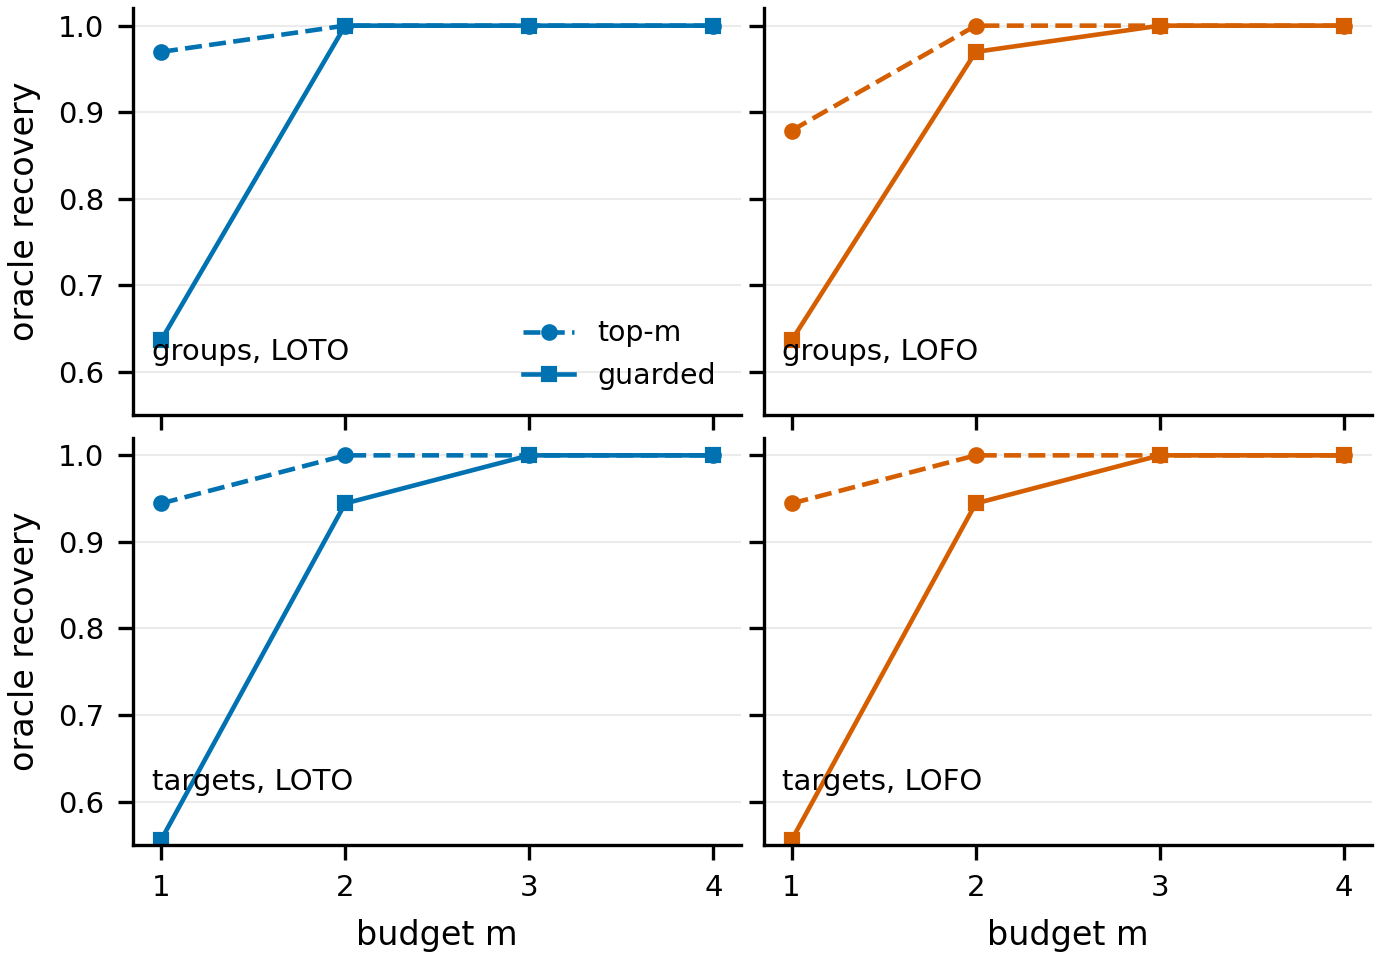
\includegraphics[width=\linewidth]{fig_budget_regret.png}
\caption{\footnotesize Oracle recovery versus materialization budget. Solid lines reserve a slot for the baseline; dashed lines are unguarded top-$m$ rankings.}
\label{fig:budget}
\end{figure}

\begin{figure}[hbt]
\centering
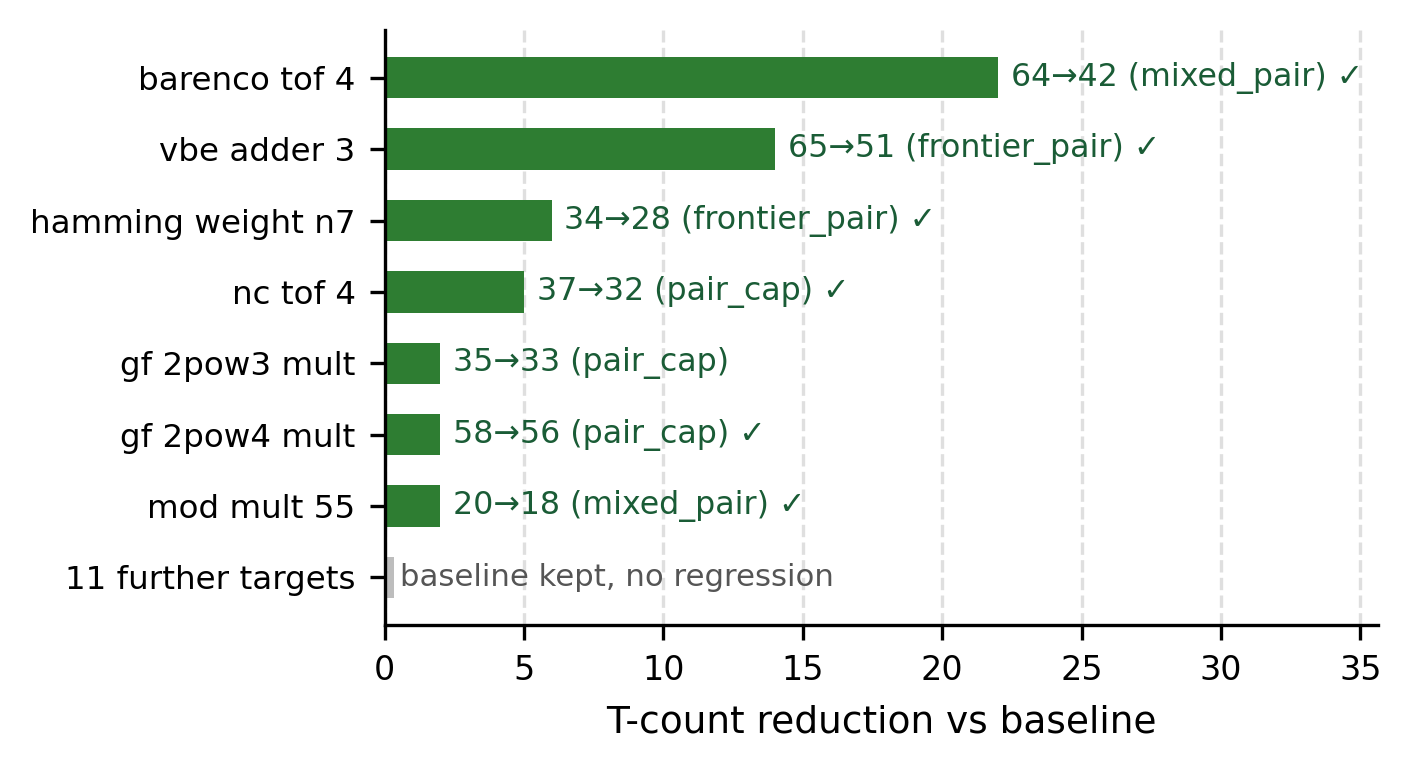
\includegraphics[width=\linewidth]{fig_tcount_reductions.png}
\caption{\footnotesize T-count reductions for the seven improved deduplicated targets under guarded top-2 selection; the aggregate row records the eleven remaining targets where the baseline is kept with no regression. Labels give baseline $\to$ selected T-count and the winning objective; \checkmark{} marks formally verified candidates.}
\label{fig:reductions}
\end{figure}

The largest verified improvements are \texttt{barenco\_tof\_4} ($64\to42$, $-34\%$, \texttt{mixed\_pair}), \texttt{vbe\_adder\_3} ($65\to51$, $-22\%$, \texttt{frontier\_pair}), and \texttt{hamming\_weight\_n7} ($34\to28$, $-18\%$, \texttt{frontier\_pair}). Several wins are modest: five of twelve group-level wins are 1--2 $T$ gates, while the largest distinct wins are 22 and 14 $T$ gates; the group-level median win is 4 $T$ gates. Certificate audit marks \texttt{mod\_mult\_55}/\texttt{mixed\_pair} certified optimal; \texttt{barenco\_tof\_4}, \texttt{vbe\_adder\_3}, \texttt{hamming\_weight\_n7}, \texttt{nc\_tof\_4}, and \texttt{gf\_2pow4\_mult} are time-limit incumbents, and the internal \texttt{gf\_2pow3\_mult} win has no retained linear-span summary. The median circuit-depth ratio is $1.0$.

\subsection{Mechanism: how the largest improvement arises}

Table~\ref{tab:case} contrasts the portfolio candidates for \texttt{barenco\_tof\_4}. The two objectives that minimize the factor count directly end at a rank-64 incumbent within the MILP budget, above the 56 $T$ gates of the original circuit. The \texttt{mixed\_pair} objective, optimizing over the \emph{same} feasible space with the same budget, reaches rank 42. This is consistent with the pairwise penalty acting as search guidance rather than merely as a post-hoc preference among equal-rank solutions. Structurally, the winning decomposition trades slightly heavier factors (mean support $2.52$ vs.\ $2.31$) for lower pairwise overlap ($0.498$ vs.\ $0.511$) and Jaccard similarity ($0.122$ vs.\ $0.136$), and it synthesizes into a shallower circuit (depth 266 vs.\ 298). This structure is rewarded by rule \eqref{eq:rule}; the broader point is that the useful objective is only observable \emph{after} decomposition, where the selection layer operates.

\begin{table}[hbt]
\centering
\caption{\footnotesize Portfolio candidates for \texttt{barenco\_tof\_4} (original circuit: 56 $T$ gates). Supp.: mean factor support weight; Ovl.: mean pairwise support overlap; Jac.: mean pairwise Jaccard similarity.}
\label{tab:case}
\footnotesize
\begin{tabular}{lccccc}
\toprule
Objective & $R$ ($=$T) & Supp. & Ovl. & Jac. & Depth \\
\midrule
\texttt{factor\_count}   & 64 & 2.31 & 0.511 & 0.136 & 298 \\
\texttt{frontier\_pair}  & 64 & 2.31 & 0.511 & 0.136 & 298 \\
\texttt{pair\_cap}       & 61 & 2.46 & 0.504 & 0.128 & 286 \\
\texttt{mixed\_pair}     & \textbf{42} & 2.52 & \textbf{0.498} & \textbf{0.122} & \textbf{266} \\
\bottomrule
\end{tabular}
\end{table}

\subsection{Which features carry the ranking signal}

Table~\ref{tab:rankaudit} compares the learned ranking with simpler controls. The learned five-feature and rank-only policies both recover the oracle on every group with zero losses; they choose different materialization sets on five groups, but the final T-counts are identical. The broader feature ablation leads to the same conclusion: the signal concentrates in $R$, and all eleven feature configurations retain zero losses because safety comes from the guard.

\begin{table}[hbt]
\centering
\caption{\footnotesize Rank audit for guarded top-2 under LOTO, group scope. The learned and rank-only policies choose different materialization sets on five groups but return identical final T-counts.}
\label{tab:rankaudit}
\footnotesize
\begin{tabular}{lccc}
\toprule
Ranking & Oracle & W/L & Max regret ($T$) \\
\midrule
learned five-feature & 33/33 & 12/0 & 0 \\
rank-only $R$        & 33/33 & 12/0 & 0 \\
alphabetical control & 30/33 & 10/0 & 6 \\
\bottomrule
\end{tabular}
\end{table}

\subsection{Effect of the guard under distribution shift}

The unguarded policy is not safe outside its training distribution: top-1 selection regresses on one instance group under LOTO and two under LOFO. The guarded policy eliminates every baseline regression in both protocols. It does not guarantee oracle recovery at fixed small budget; under LOFO, guarded top-2 misses one group oracle, but monotonicity closes that miss at budget three. Because the non-regression guarantee is structural, it extends to any future target without re-evaluation.

\subsection{Computational cost}

Wall time is dominated by the portfolio MILP decompositions (approximately 2700\,s each, embarrassingly parallel); synthesis of a single candidate takes seconds. The layer therefore requires the portfolio decompositions up front. Its practical saving at budget $m=2$ is in avoiding synthesis, audit, and verification of $K-m$ candidates; the guard itself is free.

% ============================================================
\section{Discussion and Limitations}

\textbf{Engine-agnosticism and absolute T-counts.} The baseline used here is a deterministic MILP instantiation rather than the original reinforcement-learning agent: training one agent per objective at the published scale is infeasible on academic hardware, and a deterministic engine gives every portfolio member an identical, reproducible budget, isolating the contribution of the selection layer. This resource constraint is consistent with the independent AlphaTensor-Quantum reusability report of Zen, N\"agele, and Marquardt \cite{zen2025}. Table~\ref{tab:context} makes the consequence explicit: the absolute T-counts produced by a 900--3000\,s MILP search remain well above the best published non-gadgetized results \cite{ruiz2025}, and this paper claims no state-of-the-art absolute counts. The table also shows what the layer contributes at fixed engine cost: portfolio selection closes part of the engine gap (on \texttt{mod\_mult\_55} it lands within one $T$ gate of the best published count), and where the baseline regresses below the original circuit, selection restores parity (\texttt{hamming\_weight\_n7}). The layer composes with any multi-objective decomposition engine; validating it on agent-generated portfolios is a natural next step. Repeated batteries also reveal run-to-run variation: only 5 of 12 repeated targets agree on the oracle objective, which is precisely why per-instance guarded selection is preferable to committing to a fixed objective.

\begin{table}[hbt]
\centering
\caption{\footnotesize Absolute T-counts in context (no gadgets). Orig.: unoptimized benchmark circuit; Publ.: best published non-gadgetized T-count, as compiled in \cite{ruiz2025}; Base/Sel.: MILP baseline and guarded portfolio selection.}
\label{tab:context}
\footnotesize
\begin{tabular}{lcccc}
\toprule
Circuit & Orig. & Publ. & Base & Sel. \\
\midrule
\texttt{barenco\_tof\_4}    & 56  & 23 & 64 & 42 \\
\texttt{vbe\_adder\_3}      & 70  & 19 & 65 & 51 \\
\texttt{nc\_tof\_4}         & 35  & 19 & 37 & 32 \\
\texttt{mod\_mult\_55}      & 49  & 17 & 20 & 18 \\
\texttt{gf\_2pow3\_mult}    & 63  & 29 & 35 & 33 \\
\texttt{gf\_2pow4\_mult}    & 112 & 39 & 58 & 56 \\
\texttt{hamming\_weight\_n7}& 28  & -- & 34 & 28 \\
\bottomrule
\end{tabular}
\end{table}

\textbf{Scale.} The present evaluation covers signature tensors up to size 15, which exhausts the benchmark suite below size 17. An extended battery covering tensors up to size 21, two additional circuit families, and the $K=6$ portfolio is in progress. %K6% update when consolidated.
By the structure of the guard, additional targets and objectives can add improvements but not baseline regressions.

\textbf{Rule distillation.} The closed-form rule \eqref{eq:rule} is distilled from the same dataset on which it is evaluated; the LOTO and LOFO protocols remain the out-of-sample evidence. The value of the rule lies in its interpretability and zero adoption cost.

% ============================================================
\section{Conclusion}

The choice of decomposition objective inside AlphaTensor-Quantum is target-dependent, and exploiting this dependence requires neither a better universal cost function nor a circuit-level classifier. It does require generating a portfolio of decompositions; the budgeted layer saves downstream synthesis, audit, and verification, while the reserved baseline slot gives zero T-count regressions by construction. On the present artifacts it reaches the available oracle on 33/33 groups at budget two and 18/18 targets at budget three, with a formally verified 34\% T-count reduction.

% ============================================================
\section*{Acknowledgments}

% TODO: funding, cluster (Apuana/CIn-UFPE) acknowledgment.
Computational resources were provided by the Apuana cluster at Centro de Inform\'atica, UFPE.

% ============================================================
\begin{thebibliography}{99}

\bibitem{bravyi2005}
S. Bravyi and A. Kitaev,
``Universal quantum computation with ideal Clifford gates and noisy ancillas,''
\textit{Phys. Rev. A}, vol. 71, p. 022316, 2005.

\bibitem{campbell2017}
E. T. Campbell, B. M. Terhal, and C. Vuillot,
``Roads towards fault-tolerant universal quantum computation,''
\textit{Nature}, vol. 549, pp. 172--179, 2017.

\bibitem{amy2014}
M. Amy, D. Maslov, and M. Mosca,
``Polynomial-time T-depth optimization of Clifford+T circuits via matroid partitioning,''
\textit{IEEE Trans. CAD}, vol. 33, no. 10, pp. 1476--1489, 2014.

\bibitem{heyfron2018}
L. E. Heyfron and E. T. Campbell,
``An efficient quantum compiler that reduces T count,''
\textit{Quantum Sci. Technol.}, vol. 4, p. 015004, 2018.

\bibitem{kissinger2020}
A. Kissinger and J. van de Wetering,
``Reducing the number of non-Clifford gates in quantum circuits,''
\textit{Phys. Rev. A}, vol. 102, p. 022406, 2020.

\bibitem{ruiz2025}
F. J. R. Ruiz \textit{et al.},
``Quantum circuit optimization with AlphaTensor,''
\textit{Nature Machine Intelligence}, vol. 7, pp. 374--385, 2025.

\bibitem{zen2025}
R. Zen, M. N\"agele, and F. Marquardt,
``Reusability report: Optimizing T count in general quantum circuits with AlphaTensor-Quantum,''
\textit{Nature Machine Intelligence}, 2025,
doi:10.1038/s42256-025-01166-9.

\bibitem{rice1976}
J. R. Rice,
``The algorithm selection problem,''
\textit{Advances in Computers}, vol. 15, pp. 65--118, 1976.

\bibitem{xu2008}
L. Xu, F. Hutter, H. H. Hoos, and K. Leyton-Brown,
``SATzilla: Portfolio-based algorithm selection for SAT,''
\textit{J. Artif. Intell. Res.}, vol. 32, pp. 565--606, 2008.

\bibitem{amy2018}
M. Amy,
``Towards large-scale functional verification of universal quantum circuits,''
in \textit{Proc. Quantum Physics and Logic (QPL)}, EPTCS vol. 287, pp. 1--21, 2018.

\end{thebibliography}

\end{document}
